\documentclass[a4paper,12pt]{IEEEtran}
\usepackage{graphicx}
\graphicspath{./CSC510_Assignment2_docs/}
\begin{document}

\title{CSC 510 Assignment 2 Report}
\author{Justin Oakley}
\maketitle\

\pagenumbering{arabic}
\tableofcontents
\newpage

\section{Introduction}
This report is about knowing machine learning techniques that will help in selecting suitable techniques which will provide excellent quality results for applications using the computing environment utilized in an experiment. The reason for why understanding these methods are so important in big data is because they provide higher quality data not only for machines to processes, but also for them to produce. The steps taken in order to obtain the desired data output are based on the type of learning that the machine must go through and the appropriate selection of models and algorithms that follow with that type of learning. In this assignment, supervised learning is the main type of learning that will be focused upon and the modeling strategies that will be heavily utilized in data analyzation are regression and classification. As for the information that was processed, eight different datasets were used in this assignment as well; four computer-generated datasets of differing observation amounts and two datasets based on recent graduate and graduate students, called \textit{recent-grads.csv} and \textit{grad-students.csv}, are experimented on in the regression model section, and two datasets about captured network normal and attack traffic, named \textit{nslkdd-version1.csv} and \textit{nslkdd-version2.csv}, are utilized in the classification portion. All data analyzation for the assignment is coded in the Python 3 language via the Apache Spark 2.4.0 computational engine on an Apache Hadoop cluster. With this in mind, the goal of the comprehending supervised machine learning techniques through model and algorithm selection can be achieved.

\section{Comparison of Regression Models}
The first step in developing a working knowledge of the functionality of machine learning techniques was to perform four different types of regression on four different system generated datasets of varying observation sizes, along with the \textit{recent-grads.csv} and \textit{grad-students.csv} files. The four regression models used in this portion of the assignment were standard regression, ridge regression, lasso regression, and elastic-net regression. Each type of regression are initially based on minimizing the error factor \textit{E}, then are developed in such a way that will result in each regression model's respective estimated parameter (matrix) \textit{A}, which will then be used to form the model itself in the notation, \(\textit{y} = \textit{A}\textbf{x}\) where \textbf{x} is the domain variable and \textit{y} is the response variable. In the following subsections, the individual regression models will be explored using the six datasets, then compared and contrasted to see if the change in model had any effect on the data. \underline{Note}: two datasets are one-dimensional with the only difference being that one contains twenty observations and the other has two thousand observations, while the other two datasets are made for two dimensions with the only difference being that these two sets have the same number of observations as the one-dimesional sets, respectively; the two graduate student datasets are based on employment, unemployment, and unemployment rate features of the two most popular majors per dataset.

\subsection{Standard Regression Model}
\label{sec1}
In standard regression, the estimated parameter is found by calculating: \[\textit{A} = \textit{y}\textbf{x}'(\textbf{x}\textbf{x}')^{-1}\] then plugging the matrix \textit{A} into the model equation. Using this information about standard regression and the one-dimensional data domain featuring twenty observations and two thousand observations, the following plots were generated:
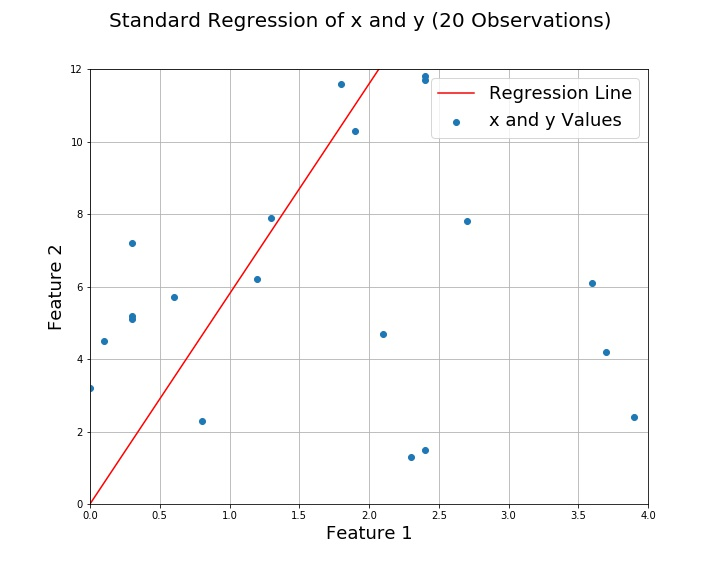
\includegraphics[width=8cm]{std_reg_1d_20_obsv} 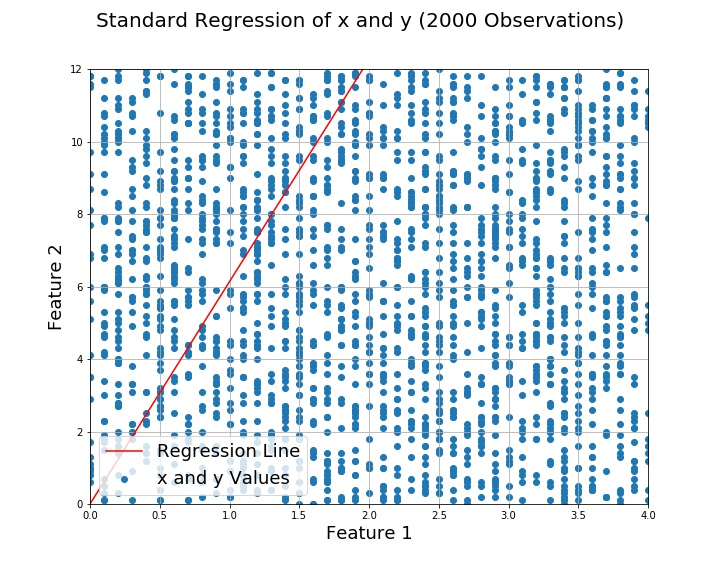
\includegraphics[width=8cm]{std_reg_1d_2000_obsv}
As for the two-dimensional data domain, the visualizations below very obvioiusly show that the linear regression model fits each set's points very well.
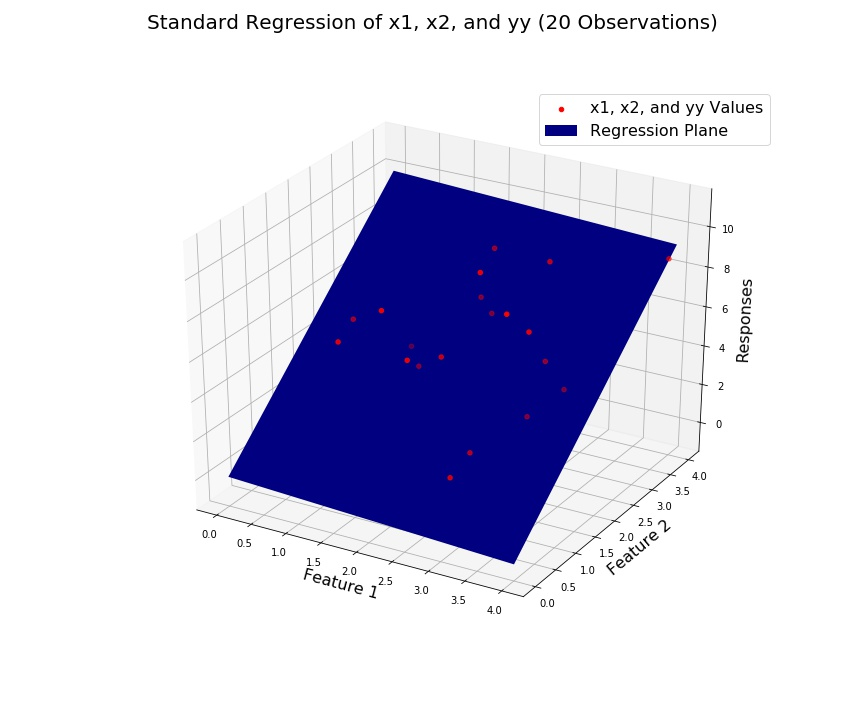
\includegraphics[width=9cm]{std_reg_2d_20_obsv} 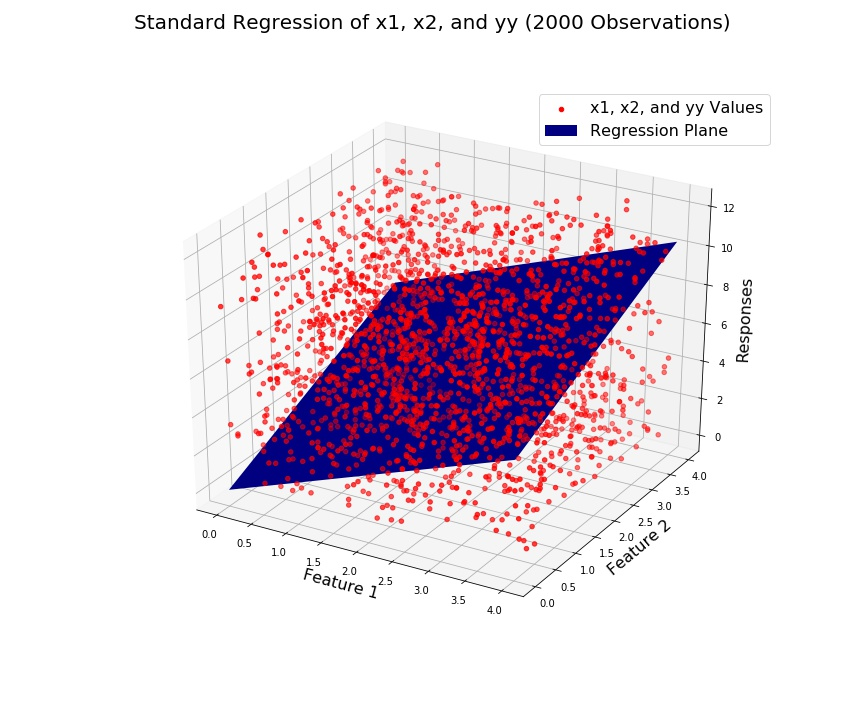
\includegraphics[width=9cm]{std_reg_2d_2000_obsv}
Moving on to the graduate student datasets, notice that despite the change in data points does not dramatically change the slope of the regression line produce from only using the one-dimensional data domain,
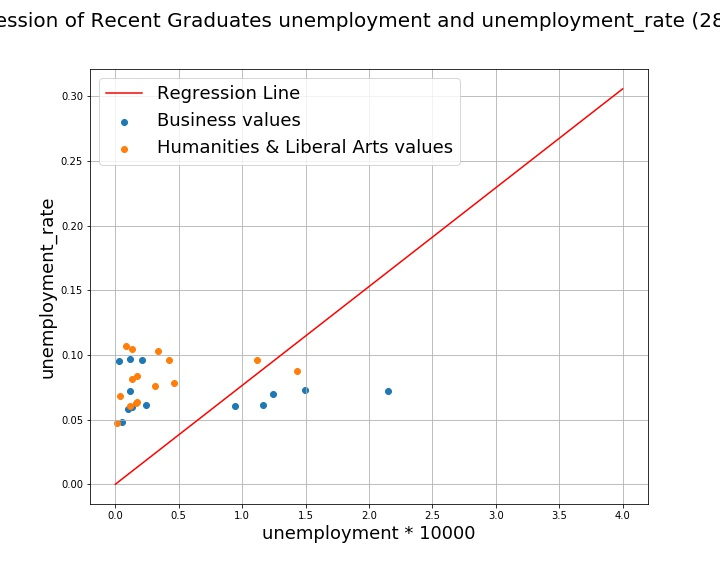
\includegraphics[width=8cm]{std_reg_1d_recent_grad} 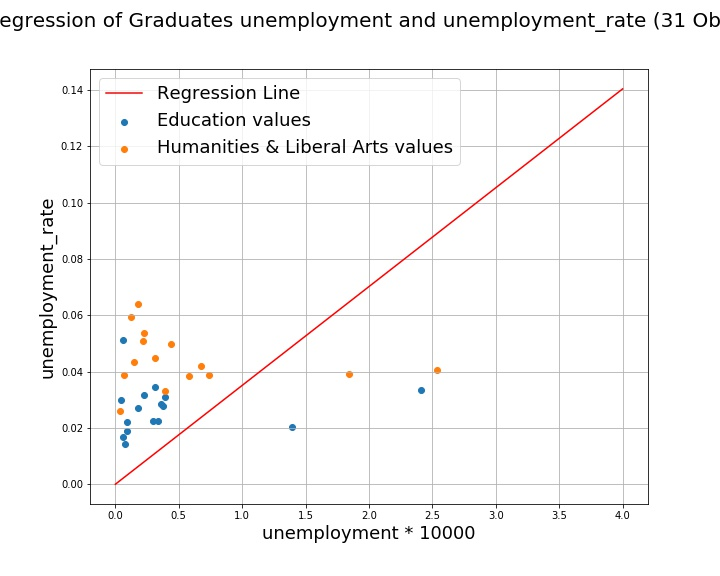
\includegraphics[width=8cm]{std_reg_1d_grad}
but when the data domain incorporates another dimension, the regression plane changes significantly.
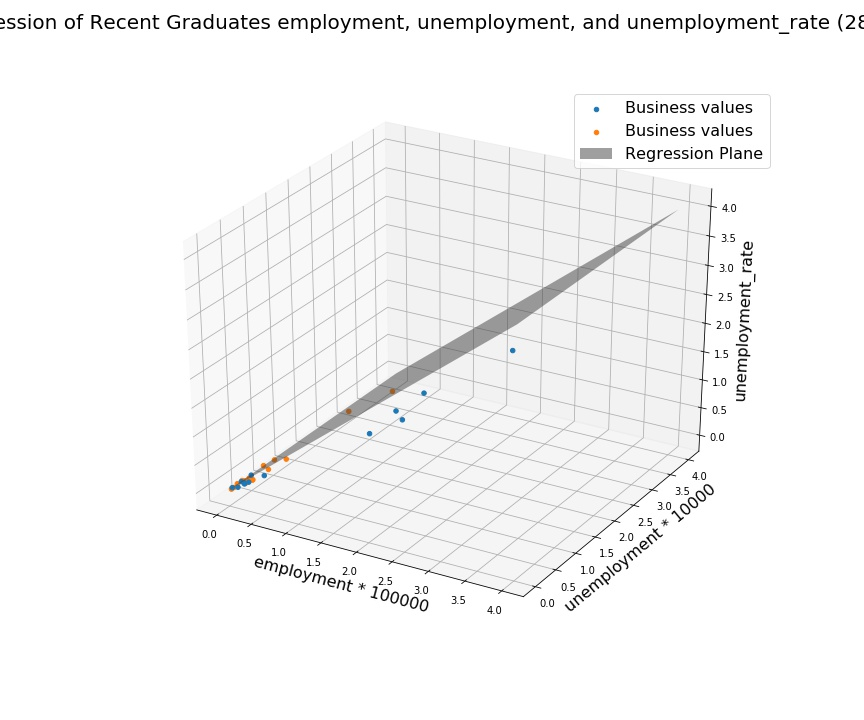
\includegraphics[width=9cm]{std_reg_2d_recent_grad} 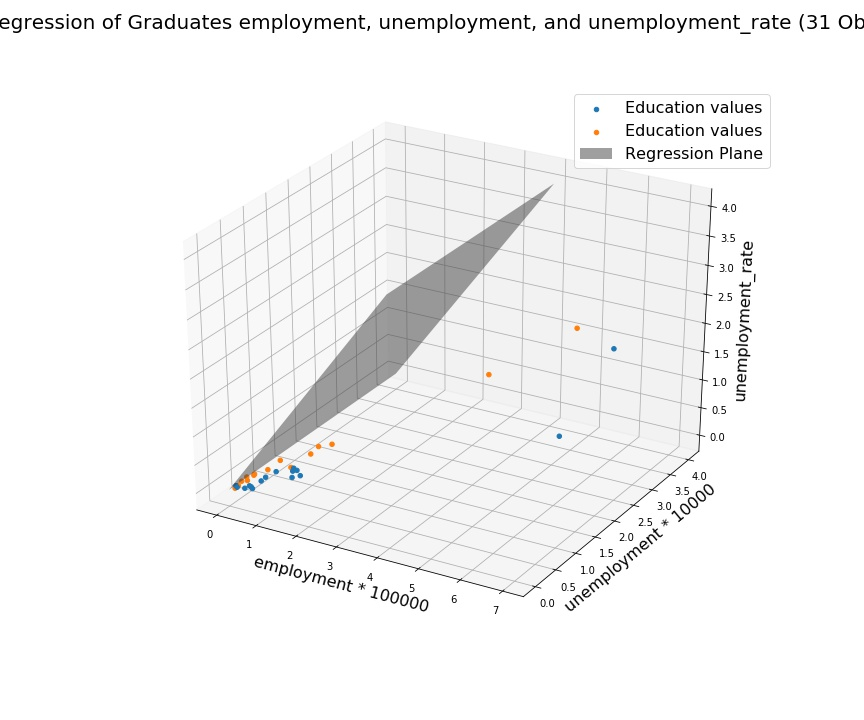
\includegraphics[width=9cm]{std_reg_2d_grad}
What this means is that both datasets 

\subsection{Ridge Regression Model}
\label{sec2}

\subsection{Lasso Regression Model}
\label{sec3}

\subsection{Elastic-Net Regression Model}
\label{sec4}

\subsection{Regression Model Overview}
\label{sec5}

\section{Network Intrusion Dataset and Random Forest}

\subsection{Basic Statistics of the Network Intrusion Dataset}
\label{sec6}

\subsection{Classification of the Network Intrusion Dataset}
\label{sec7}

\end{document}